Given Equation can be written as:
\begin{align}
    f(x)=(2x-1)^2+3=4x^2-4x+4
\end{align}
   A function is said to be convex if following inequality is true:
    \begin{align}
        \lambda f(x_1)+(1-\lambda) f(x_2) \geq f(\lambda x_1+(1-\lambda) x_2)
    \end{align}
    and for $\lambda \in [0,1]$
\begin{align}
&\lambda(4x_1^2-4x_1+4)+(1-\lambda)((4x_2^2-4x_2+4) \geq \nonumber \\ 
&4(\lambda x_1 +(1-\lambda )x_2)^2-4(\lambda x_1 +(1-\lambda )x_2)+4\\
&x_1^2(4\lambda-4\lambda^2)+x_2^2(4\lambda-4\lambda^2)-2x_1x_2(4\lambda-4\lambda^2) \geq 0\\
&4\lambda(1-\lambda)(x_1-x_2)^2 \geq 0
\end{align}
The above inequality is always true for all values from the domain. Hence the given function f(x) is convex.
%\begin{align}
%	\vec{x}^T\myvec{4&0\\0&0}\vec{x}  + \myvec{-4&0}\vec{x} +4 = 0
%\end{align}


    Using gradient descent method,
    \begin{align}
    x_n=x_{n-1}-\mu\frac{df(x)}{dx} \label{eq:solutions/5/2/1/1/eq2}
    \end{align}
    Here, $\mu$ is learning rate.\\
    \begin{align}
    \frac{df(x)}{dx}=8x-4 \label{eq:solutions/5/2/1/1/eq3}
\end{align}
After substituting \ref{eq:solutions/5/2/1/1/eq3} in \ref{eq:solutions/5/2/1/1/eq2} we get:
\begin{align}
x_n=x_{n-1}-\mu( 8x_{n-1}-4)\label{eq:solutions/5/2/1/1/eq4}
\end{align}
In equation \eqref{eq:solutions/5/2/1/1/eq4}, $\mu$ is a variable parameter known as step size. $x_{n+1}$ is the next position. The minus sign refers to the minimization part of gradient descent. Assume, $\mu=0.01$, $x_0=2$ and following the above method, we keep doing iterations until $x_{n+1}-x_{n}$ becomes less than the value of precision we have chosen.
\begin{align}
    x_n=0.5
\end{align}
The following python code computes the minimum value as plotted in Fig. \ref{eq:solutions/5/2/1/1/fig:5.1}. Hence, The minimum value of $f(x)$ at $x=0.5$ is 3.
	\begin{lstlisting}
	./codes/Assignment_4.py
	\end{lstlisting}
		\begin{figure}[!ht]
	\centering
	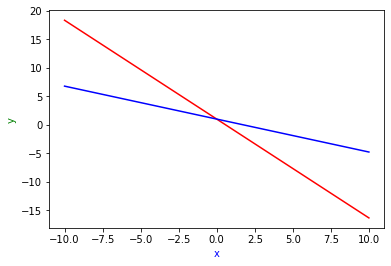
\includegraphics[width=\columnwidth]{./solutions/5/2/1/1/Figure_1.png}
	\caption{Plot of the given polynomial}
	\label{eq:solutions/5/2/1/1/fig:5.1}	
	\end{figure}

